%-*-latex-*-
\sectionthree{Implementation}
\begin{python0}
from solutions import *; clear()
\end{python0}


There are many different ways to implement a tree node.
\begin{tightlist}
  \li The node might or might not have a pointer back to the parent. (And as stated
  in class the parent pointer is usually not necessary.)
  \li The children (or rather pointers to the children nodes) can be
  collected together in different ways.
  For instance they can form an array, a vector or a linked list (singly linked or doubly
  linked). If the maximum number of children (i.e., the branching factor)
  is small, then sometimes you can have a number of pointer instance variables
  directly attached to the node object rather than putting the pointers
  into a container.
  This is usually the case for binary trees.
\end{tightlist}

\newpage
\subsection{Vector of children}

For a general tree, one way to implement a tree node is to do this:
\begin{console}
class Node 
{
private:
    int key_;
    std::vector< Node * > child_;
};
\end{console}
(Of course instead of keeping an \verb!int! for each node, you might
want to keep other values.)
The \verb!child_! member variable will allow a node to point to any number
of children.

For the case of a $k$--ary tree, if $k$ is small,
instead of using some kind of container class, 
it's also common to use a fixed size array:
\begin{console}
const int k = 4;
class Node 
{
private:
    int key_;
    Node * child_[k];
};
\end{console}
Of course in the case when a node does not have a \lq\lq child 2'',
then \verb!child_[2]! is \verb!NULL!.

In the case of a binary tree, it's common to see this:
\begin{console}
class Node 
{
private:
    int key_;
    Node * left_;
    Node * right_;
};
\end{console}

\newpage
\begin{ex}
  Here a tree (the first one in this section):
  {\small \begin{console}[frame=single,fontsize=\small]
[student@localhost 350-hashtable] g++ main.cpp; ./a.out
hash of
42: 42
42: 42
-1: 18446744073709551615
3.14: 5464867211497793177
0.0: 6369015886390043782
'a': 97
true: 1
"hello world": 5577293430985752569
\end{console}
}

  
The key values are characters.
Construct the above tree with this
\begin{Verbatim}[frame=single]
class Node
{
private:
    char key_;
    std::vector< Node * > child_;
}
\end{Verbatim}


Here's a picture of the memory model (using the given class)
representing the node with key \verb!'a'!.

\begin{center}
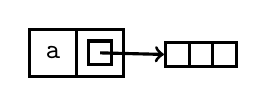
\begin{tikzpicture}

\draw (0.3, 0.3)
  node[draw, line width=0.04cm, , color=black,
       rounded corners=0cm, inner sep=0cm] {

\begin{minipage}[t][0.6cm]{0.6cm}
\mbox{}

\end{minipage}

};\draw (0.3, 0.3) node[color=black] {{\texttt{a}}};
\draw (0.8999999999999999, 0.3)
  node[draw, line width=0.04cm, , color=black,
       rounded corners=0cm, inner sep=0cm] {

\begin{minipage}[t][0.6cm]{0.6cm}
\mbox{}

\end{minipage}

};
\draw (0.9, 0.3)
  node[draw, line width=0.04cm, , color=black,
       rounded corners=0cm, inner sep=0cm] {

\begin{minipage}[t][0.3cm]{0.3cm}
\mbox{}

\end{minipage}

};
\draw (1.88, 0.28)
  node[draw, line width=0.04cm, , color=black,
       rounded corners=0cm, inner sep=0cm] {

\begin{minipage}[t][0.3cm]{0.3cm}
\mbox{}

\end{minipage}

};
\draw (2.1799999999999997, 0.28)
  node[draw, line width=0.04cm, , color=black,
       rounded corners=0cm, inner sep=0cm] {

\begin{minipage}[t][0.3cm]{0.3cm}
\mbox{}

\end{minipage}

};
\draw (2.48, 0.28)
  node[draw, line width=0.04cm, , color=black,
       rounded corners=0cm, inner sep=0cm] {

\begin{minipage}[t][0.3cm]{0.3cm}
\mbox{}

\end{minipage}

};\draw[line width=0.04cm,black,->] (0.9,0.3) to  (1.71,0.28);
\end{tikzpicture}

\end{center}



The first box is holds the key value -- the box is \texttt{key\_}.
The second box is \texttt{child\_} which is a \texttt{std::vector} object
which of course models a dynamic array and therefore
contains a pointer to an array (of \texttt{Node *} values).
The first pointer of this dynamic array  of pointers points to a node with key value
\verb!'b'!,
the second points to a node with key value \verb!'c'!, and 
the third points to a node with key value \verb!'d'!.



Here's part of the memory model of the above tree:

\begin{center}
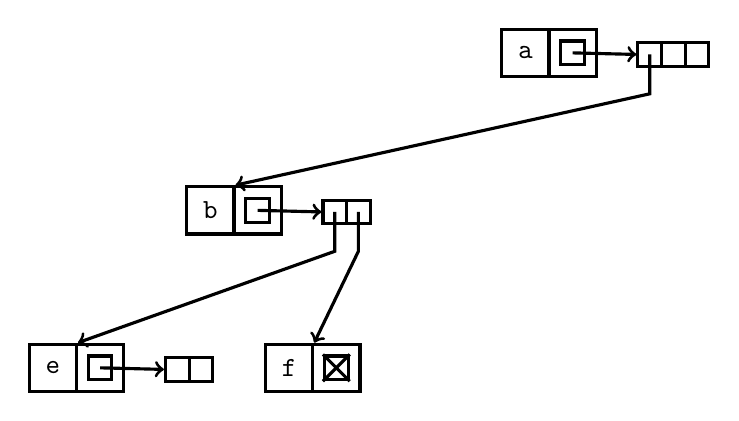
\begin{tikzpicture}

\draw (0.3, 0.3)
  node[draw, line width=0.04cm, , color=black,
       rounded corners=0cm, inner sep=0cm] {

\begin{minipage}[t][0.6cm]{0.6cm}
\mbox{}

\end{minipage}

};\draw (0.3, 0.3) node[color=black] {{\texttt{a}}};
\draw (0.8999999999999999, 0.3)
  node[draw, line width=0.04cm, , color=black,
       rounded corners=0cm, inner sep=0cm] {

\begin{minipage}[t][0.6cm]{0.6cm}
\mbox{}

\end{minipage}

};
\draw (0.9, 0.3)
  node[draw, line width=0.04cm, , color=black,
       rounded corners=0cm, inner sep=0cm] {

\begin{minipage}[t][0.3cm]{0.3cm}
\mbox{}

\end{minipage}

};
\draw (1.88, 0.28)
  node[draw, line width=0.04cm, , color=black,
       rounded corners=0cm, inner sep=0cm] {

\begin{minipage}[t][0.3cm]{0.3cm}
\mbox{}

\end{minipage}

};
\draw (2.1799999999999997, 0.28)
  node[draw, line width=0.04cm, , color=black,
       rounded corners=0cm, inner sep=0cm] {

\begin{minipage}[t][0.3cm]{0.3cm}
\mbox{}

\end{minipage}

};
\draw (2.48, 0.28)
  node[draw, line width=0.04cm, , color=black,
       rounded corners=0cm, inner sep=0cm] {

\begin{minipage}[t][0.3cm]{0.3cm}
\mbox{}

\end{minipage}

};\draw[line width=0.04cm,black,->] (0.9,0.3) to  (1.71,0.28);

\draw (-3.6999999999999997, -1.7)
  node[draw, line width=0.04cm, , color=black,
       rounded corners=0cm, inner sep=0cm] {

\begin{minipage}[t][0.6cm]{0.6cm}
\mbox{}

\end{minipage}

};\draw (-3.6999999999999997, -1.7) node[color=black] {{\texttt{b}}};
\draw (-3.0999999999999996, -1.7)
  node[draw, line width=0.04cm, , color=black,
       rounded corners=0cm, inner sep=0cm] {

\begin{minipage}[t][0.6cm]{0.6cm}
\mbox{}

\end{minipage}

};
\draw (-3.0999999999999996, -1.7)
  node[draw, line width=0.04cm, , color=black,
       rounded corners=0cm, inner sep=0cm] {

\begin{minipage}[t][0.3cm]{0.3cm}
\mbox{}

\end{minipage}

};
\draw (-2.12, -1.7200000000000002)
  node[draw, line width=0.04cm, , color=black,
       rounded corners=0cm, inner sep=0cm] {

\begin{minipage}[t][0.3cm]{0.3cm}
\mbox{}

\end{minipage}

};
\draw (-1.8199999999999998, -1.7200000000000002)
  node[draw, line width=0.04cm, , color=black,
       rounded corners=0cm, inner sep=0cm] {

\begin{minipage}[t][0.3cm]{0.3cm}
\mbox{}

\end{minipage}

};\draw[line width=0.04cm,black,->] (-3.1,-1.7) to  (-2.29,-1.72);

\draw (-5.7, -3.6999999999999997)
  node[draw, line width=0.04cm, , color=black,
       rounded corners=0cm, inner sep=0cm] {

\begin{minipage}[t][0.6cm]{0.6cm}
\mbox{}

\end{minipage}

};\draw (-5.7, -3.6999999999999997) node[color=black] {{\texttt{e}}};
\draw (-5.1, -3.6999999999999997)
  node[draw, line width=0.04cm, , color=black,
       rounded corners=0cm, inner sep=0cm] {

\begin{minipage}[t][0.6cm]{0.6cm}
\mbox{}

\end{minipage}

};
\draw (-5.1, -3.7)
  node[draw, line width=0.04cm, , color=black,
       rounded corners=0cm, inner sep=0cm] {

\begin{minipage}[t][0.3cm]{0.3cm}
\mbox{}

\end{minipage}

};
\draw (-4.119999999999999, -3.72)
  node[draw, line width=0.04cm, , color=black,
       rounded corners=0cm, inner sep=0cm] {

\begin{minipage}[t][0.3cm]{0.3cm}
\mbox{}

\end{minipage}

};
\draw (-3.8199999999999994, -3.72)
  node[draw, line width=0.04cm, , color=black,
       rounded corners=0cm, inner sep=0cm] {

\begin{minipage}[t][0.3cm]{0.3cm}
\mbox{}

\end{minipage}

};\draw[line width=0.04cm,black,->] (-5.1,-3.7) to  (-4.29,-3.72);

\draw (-2.7, -3.6999999999999997)
  node[draw, line width=0.04cm, , color=black,
       rounded corners=0cm, inner sep=0cm] {

\begin{minipage}[t][0.6cm]{0.6cm}
\mbox{}

\end{minipage}

};\draw (-2.7, -3.6999999999999997) node[color=black] {{\texttt{f}}};
\draw (-2.1, -3.6999999999999997)
  node[draw, line width=0.04cm, , color=black,
       rounded corners=0cm, inner sep=0cm] {

\begin{minipage}[t][0.6cm]{0.6cm}
\mbox{}

\end{minipage}

};
\draw (-2.1, -3.7)
  node[draw, line width=0.04cm, , color=black,
       rounded corners=0cm, inner sep=0cm] {

\begin{minipage}[t][0.3cm]{0.3cm}
\mbox{}

\end{minipage}

};\draw[line width=0.04cm,black] (-2.27,-3.53) to  (-1.93,-3.87);
\draw[line width=0.04cm,black] (-1.93,-3.53) to  (-2.27,-3.87);
\draw[line width=0.04cm,black,->] (1.88,0.28) to  (1.88,-0.22) to  (-3.38,-1.38);
\draw[line width=0.04cm,black,->] (-2.12,-1.72) to  (-2.12,-2.22) to  (-5.38,-3.38);
\draw[line width=0.04cm,black,->] (-1.82,-1.72) to  (-1.82,-2.22) to  (-2.38,-3.38);
\end{tikzpicture}

\end{center}



The pointers in the node with keys \verb!'f'! is \verb!NULL!
since the \verb!std::vector! inside the node models array of size 0,
i.e., I'm assuming that the pointer in the \verb!std::vector! objects
have not been allocated memory yet.

Complete the picture. Solution on next page.

\newpage


\begin{center}
\begin{tikzpicture}[>=triangle 60,shorten >=0.5pt,node distance=2cm,auto,initial text=, double distance=2pt]
\node[state] (A) at (  0,  0) {$\{q_0\}$};
\node[state] (B) at (  3,  0) {$\{\}$};

\path[->]

;
\end{tikzpicture}
\end{center}
    


\begin{ex}
First add an obvious constructor to this class.
Assume that the values in all the \verb!child_!
vectors are not \texttt{NULL}.
Add a method \texttt{child(int)} that does the obvious (see
the code below).
The three nodes on the bottom left of the above diagram is
already constructed for you.

\begin{Verbatim}[frame=single]
int main()
{
    Node * nk = new Node('k');
    Node * nl = new Node('l');
    Node * ne = new Node('e');
    ne->child(0) = nk; // i.e., ne->child_[0] = nk
    ne->child(1) = nl; // i.e., ne->child_[1] = nl
    
    return 0;
}
\end{Verbatim}
\qed
\end{ex}
\end{ex}



\newpage
\subsection{List of children}

Depending on how the children 
are going to be processed, 
you might want to use something other than 
\verb!std::vector!.
For instance, here's another option:
\begin{console}
class Node 
{
private:
    int key_;
    std::list< Node * > child_;
};
\end{console}
where a node has a doubly-linked list of 
pointers to \verb!Node!.
You can also use circular list.
In the case of the undirected version (think of an edge
as bi-directional so that it allows one to go up or down the tree), 
you might see this:
\begin{console}
class Node 
{
private:
    int key_;
    Node * parent_;
    std::list< Node * > child_;
};
\end{console}
Frequently, it's not necessary to keep information on how to get back to 
the parent in the node since most tree 
computations start with the root and when you 
\lq\lq go down'', you keep information of the parents (i.e. where
you came from) somewhere such as a stack.

\begin{ex}
  Here a tree (the first one in this section):

  
\begin{longtable}{|r||r|r|r|r|r|}
\hline 
         & $w_1$ & $w_2$ & $w_3$ & $w_4$ & $\ldots$ \\ \hline \hline 
$M_1$    &       &       &       &       &          \\ \hline 
$M_2$    &       &       &       &       &          \\ \hline 
$M_3$    &       &       &       &       &          \\ \hline 
$M_4$    &       &       &       &       &          \\ \hline 
$\ldots$ &       &       &       &       &          \\ \hline 
\end{longtable}
        

  
The key values are characters.
Construct the above tree with this
\begin{Verbatim}[frame=single]
class Node
{
private:
int key_;
std::list< Node * > child_;
}
\end{Verbatim}

The following diagram shows the memory model when the above class
is used to model the tree:


\begin{longtable}{|r||r|r|r|r|r|}
\hline 
         & $w_1$ & $w_2$ & $w_3$ & $w_4$ & $\ldots$ \\ \hline \hline 
$M_1$    & 0     & 0     & 1     & 0     & ...      \\ \hline 
$M_2$    & 1     & 0     & 1     & 1     & ...      \\ \hline 
$M_3$    & 0     & 1     & 1     & 1     & ...      \\ \hline 
$M_4$    & 1     & 0     & 1     & 1     & ...      \\ \hline 
$\ldots$ &       &       &       &       &          \\ \hline 
\end{longtable}
        


Each node is representation by a box containing two boxes
where the first box contains the value of the key and the second
box contains a doubly linked list.
For the doubly linked list, I'm not drawing the pointer to
head and pointer to tail just to simplify the diagram.
If the linked list is empty, I draw the second box empty.

\qed
\end{ex}


\newpage
\subsection{Binary trees}

Recall that for the case of a $k$--ary tree,
if $k$ is small,
instead of using some kind of container class, 
it's also common to use a fixed size array:
\begin{console}
const int k = 4;
class Node 
{
private:
    int key_;
    Node * child_[k];
};
\end{console}
Now in the case of a \textit{binary} tree,
instead of using an array of only two pointers for the children, 
it's common to see this:
\begin{console}
class Node 
{
private:
    int key_;
    Node * parent_;
    Node * left_;
    Node * right_;
};
\end{console}
i.e., you hardcode the pointers (to children) into the node object.

\begin{ex}
Start with this node class:
\begin{console}
class Node
{
private:
    int key_;
    Node * parent_;
    Node * left_;
    Node * right_;
};
\end{console}

In the case of $k$--ary tree node when you have an array for the children pointers,
of course you can loop over children pointers.
For binary tree nodes like the above, you can't but this is not a problem
since we usually do not loop over them anyway.

\end{ex}
Write a constructor so that you can do this:
\begin{console}
Node * p2 = new Node(2);
\end{console}
and this
\begin{console}
Node * p2 = new Node(2, parent_pointer);
\end{console}
and this
\begin{console}
Node * p2 = new Node(2, parent_pointer,
                     left_child_ptr, right_child_ptr);
\end{console}

\begin{comment}
It should look like this:
\begin{console}
...
    Node(int key=0,
         Node * parent=NULL,
         Node * left=NULL, Node * right=NULL)
        : key_(key),
          parent_(parent),
          left_(left), right_(right)
    {}
...
\end{console}
\end{comment}
If a \verb!node! is an object of the above class, 
when you do
\begin{Verbatim}[commandchars=\\\{\},frame=single]
std::cout << node << std::endl;
\end{Verbatim}
you will get this output:
{\small
\begin{Verbatim}[frame=single, commandchars=\\\{\}]
<Node 0x97900b0 key:5, parent:0, left:0x9790050, right:0x9790068>
\end{Verbatim}
}



\newpage
\subsection{Tree class}

Of course once you have the definition of a tree node, 
the important things left would be how to link up the nodes
(just like the case of linked lists, double or single),
how to delete nodes, 
how to run through the tree to search for things, etc.

Now, it's not too shocking that if you have a class for the 
tree, you just need to have access to the root of the tree:
{\small
\begin{Verbatim}[frame=single]
class Tree
{
private:
    Node * root_;
};
\end{Verbatim}
}

Since it's just a single node (or pointer or reference to a node),
frequently, you won't see tree classes at all.
Many books or data structure libraries will just have tree node classes
and have function/methods attached to the node class.
However if you have a tree class, then you can store tree-level
information in a tree object.
For instance
{\small
\begin{Verbatim}[frame=single]
class Tree
{
private:
    Node * root_;
    int size_;
};
\end{Verbatim}
}
where \verb!size_! contains the number of nodes in the tree.
There are also tree level operations (instead of node level operations)
that you attach to a tree class.
For instance you can have a node level comparison operator
{\small
\begin{Verbatim}[frame=single]
class TreeNode
{
public:
    ...
    bool & operator=(const TreeNode & n) const
    {
        ...
    }
    ...
};
\end{Verbatim}
}
and a class
level comparison operator
{\small
\begin{Verbatim}[frame=single]
class Tree
{
public:
    ...
    bool operator==(const Tree & t) const
    {
        ...
    }
    ...
};
\end{Verbatim}
}
In this case, the assignment operator at the node level,
say you compute \texttt{n1 == n2},
then this is the same as comparing the key or \texttt{n1}
again the key of \texttt{n2}.
However the comparison operator at the tree level,
say you have the boolean expression \texttt{t1 == t2},
will have to compare the tree structure of \texttt{t1}
(i.e., the layout of the nodes)
against the structure of \texttt{t2} and at the
same time comparing their keys.

In some cases where a tree is self-organizing, you only need to
specify values to be added or to be removed from whole tree.
(Example: binary search trees, AVL trees, quadtrees, etc. See later notes.).
In those cases have a tree class is very helpful.
You would envision that a tree is used like this:
\begin{console}
Tree tree;
tree.insert(5);
tree.insert(7);
tree.insert(2);
tree.insert(0);
...
tree.insert(42);
\end{console}
This is similar to for instance a stack or queue which are self-organizing data
structures.

There are however many cases where you have to manually
decide where to attach nodes:
\begin{console}
Tree tree;
...
Node * p = tree.find(42);
if (p->left() == NULL)
{
    p->insert_left(51);  
}
\end{console}
For instance in the case of expression trees (trees from
expressions like \texttt{1 + 2 * 3}),
you have to build the tree in a specific way.
You can just insert \texttt{2}, insert \texttt{+}, etc.
You have to use a specific algorithm to build the expression tree yorself.
